% Тип документа
\documentclass[a4paper,12pt]{extarticle}

% Шрифты, кодировки, символьные таблицы, переносы
\usepackage{cmap}
\usepackage[T2A]{fontenc}
\usepackage[utf8x]{inputenc}
\usepackage[russian]{babel}

% Это пакет -- хитрый пакет, он нужен но не нужен
\usepackage[mode=buildnew]{standalone}

\usepackage
	{
		% Дополнения Американского математического общества (AMS)
		amssymb,
		amsfonts,
		amsmath,
		amsthm,
		% misccorr,
		% 
		% Графики и рисунки
		wrapfig,
		graphicx,
		subcaption,
		float,
		tikz,
		tikz-3dplot,
		caption,
		csvsimple,
		color,
		booktabs,
		pgfplots,
		pgfplotstable,
		geometry,
		% 
		% Таблицы, списки
		makecell,
		multirow,
		indentfirst,
		%
		% Интегралы и прочие обозначения
		ulem,
		esint,
		esdiff,
		% 
		% Колонтитулы
		fancyhdr,
	}  


% Обводка текста в TikZ
\usepackage[outline]{contour}

% Увеличенный межстрочный интервал, французские пробелы
\linespread{1.3} 
\frenchspacing 

 
\usetikzlibrary
	{
		decorations.pathreplacing,
		decorations.pathmorphing,
		patterns,
		calc,
		scopes,
		arrows,
		fadings,
		through,
		shapes.misc,
		arrows.meta,
		3d,
		quotes,
		angles,
		babel
	}


\tikzset{
	force/.style=	{
		>=latex,
		draw=blue,
		fill=blue,
				 	}, 
	%				 	
	axis/.style=	{
		densely dashed,
		blue,
		line width=1pt,
		font=\small,
					},
	%
	th/.style=	{
		line width=1pt},
	%
	acceleration/.style={
		>=open triangle 60,
		draw=magenta,
		fill=magenta,
					},
	%
	inforce/.style=	{
		force,
		double equal sign distance=2pt,
					},
	%
	interface/.style={
		pattern = north east lines, 
		draw    = none, 
		pattern color=gray!60,
					},
	cross/.style=	{
		cross out, 
		draw=black, 
		minimum size=2*(#1-\pgflinewidth), 
		inner sep=0pt, outer sep=0pt,
					},
	%
	cargo/.style=	{
		rectangle, 
		fill=black!70, 
		inner sep=2.5mm,
					},
	%
	caption/.style= {
		midway,
		fill=white!20, 
		opacity=0.9
					},
	%
	}

\newenvironment{tikzpict}
    {
	    \begin{figure}[htbp]
		\centering
		\begin{tikzpicture}
    }
    { 
		\end{tikzpicture}
		% \caption{caption}
		% \label{fig:label}
		\end{figure}
    }


\newcommand{\vbLabel}[3]{\draw ($(#1,#2)+(0,5pt)$) -- ($(#1,#2)-(0,5pt)$) node[below]{#3}}
\newcommand{\vaLabel}[3]{\draw ($(#1,#2)+(0,5pt)$) node[above]{#3} -- ($(#1,#2)-(0,5pt)$) }

\newcommand{\hrLabel}[3]{\draw ($(#1,#2)+(5pt,0)$) -- ($(#1,#2)-(5pt,0)$) node[right, xshift=1em]{#3}}
\newcommand{\hlLabel}[3]{\draw ($(#1,#2)+(5pt,0)$) node[left, xshift=-1em]{#3} -- ($(#1,#2)-(5pt,0)$) }



\newcommand\zi{^{\,*}_i}
\newcommand\sumn{\sum_{i=1}^{N}}

\tikzset{
	coordsys/.style={scale=1.8,x={(1.1cm,-0cm)},y={(0.5cm,1cm)}, z={(0cm,0.8cm)}},
	coordsys/.style={scale=1.5,x={(0cm,0cm)},y={(1cm,0cm)}, z={(0cm,1cm)}}, 
	coordsys/.style={scale=1.5,x={(1cm,0cm)},y={(0cm,1cm)}, z={(0cm,0cm)}}, 
}

\usepgfplotslibrary{units}


% Draw line annotation
% Input:
%   #1 Line offset (optional)
%   #2 Line angle
%   #3 Line length
%   #5 Line label
% Example:
%   \lineann[1]{30}{2}{$L_1$}

\newcommand{\lineann}[4][0.5]{%
    \begin{scope}[rotate=#2, blue,inner sep=2pt, ]
        \draw[dashed, blue!40] (0,0) -- +(0,#1)
            node [coordinate, near end] (a) {};
        \draw[dashed, blue!40] (#3,0) -- +(0,#1)
            node [coordinate, near end] (b) {};
        \draw[|<->|] (a) -- node[fill=white, scale=0.8] {#4} (b);
    \end{scope}
}

\newcommand{\lineannn}[4][0.5]{%
    \begin{scope}[rotate=#2, blue,inner sep=2pt, ]
        \draw[dashed, blue!40] (0,0) -- +(0,#1)
            node [coordinate, near end] (a) {};
        \draw[dashed, blue!40] (#3,0) -- +(0,#1)
            node [coordinate, near end] (b) {};
        % \draw[color=white, color=blue] (a) -- node[fill=white, scale=0.8] {#4} (b);
        \draw[->|] (a)++(-0.3,0) -- (a);
        \draw[->|] (b)++(0.3,0) coordinate (xx) -- (b);
        \draw (xx) node[fill=white, scale=0.8, right] {#4};
    \end{scope}
}

% Круговая стрелка относительно центра (дуга из центра)
\tikzset{
  pics/carc/.style args={#1:#2:#3}{
    code={
      \draw[pic actions] (#1:#3) arc(#1:#2:#3);
    }
  },
  dash/.style={
  	dash pattern=on 5mm off 5mm
  }
}

% Среднее <#1>
\newcommand{\mean}[1]{\langle#1\rangle}

\pgfplotsset{
    % most recent feature set of pgfplots
    compat=newest,
}

% const прямым шрифтом
\newcommand\ct[1]{\text{\rmfamily\upshape #1}}
\newcommand*{\const}{\ct{const}}


\usepackage[europeanresistors,americaninductors]{circuitikz}

% Style to select only points from #1 to #2 (inclusive)
\pgfplotsset{select/.style 2 args={
    x filter/.code={
        \ifnum\coordindex<#1\def\pgfmathresult{}\fi
        \ifnum\coordindex>#2\def\pgfmathresult{}\fi
    }
}}


\usepackage{array}



%%%%%%%%%%%%%%%%%%%%%%%%%%%%%%%%%%%%%%%%%%%%%%%%%
\makeatletter
\newif\if@gather@prefix 
\preto\place@tag@gather{% 
  \if@gather@prefix\iftagsleft@ 
    \kern-\gdisplaywidth@ 
    \rlap{\gather@prefix}% 
    \kern\gdisplaywidth@ 
  \fi\fi 
} 
\appto\place@tag@gather{% 
  \if@gather@prefix\iftagsleft@\else 
    \kern-\displaywidth 
    \rlap{\gather@prefix}% 
    \kern\displaywidth 
  \fi\fi 
  \global\@gather@prefixfalse 
} 
\preto\place@tag{% 
  \if@gather@prefix\iftagsleft@ 
    \kern-\gdisplaywidth@ 
    \rlap{\gather@prefix}% 
    \kern\displaywidth@ 
  \fi\fi 
} 
\appto\place@tag{% 
  \if@gather@prefix\iftagsleft@\else 
    \kern-\displaywidth 
    \rlap{\gather@prefix}% 
    \kern\displaywidth 
  \fi\fi 
  \global\@gather@prefixfalse 
} 
\newcommand*{\beforetext}[1]{% 
  \ifmeasuring@\else
  \gdef\gather@prefix{#1}% 
  \global\@gather@prefixtrue 
  \fi
} 
\makeatother
%%%%%%%%%%%%%%%%%%%%%%%%%%%%%%%%%%%%%%%%%%%%%%%%%

\geometry		
	{
		left			=	2cm,
		right 			=	2cm,
		top 			=	3cm,
		bottom 			=	3cm,
		bindingoffset	=	0cm
	}

%%%%%%%%%%%%%%%%%%%%%%%%%%%%%%%%%%%%%%%%%%%%%%%%%%%%%%%%%%%%%%%%%%%%%%%%%%%%%%%

\def\labauthors{Понур К.А., Сарафанов Ф.Г., Сидоров Д.А.}
\def\labgroup{420}
\def\labnumber{222}
\def\labtheme{Изучение разряда неоновой лампы}

	%применим колонтитул к стилю страницы
\pagestyle{fancy} 
	%очистим "шапку" страницы
\fancyhead{} 
	%слева сверху на четных и справа на нечетных
\fancyhead[R]{\labauthors} 
	%справа сверху на четных и слева на нечетных
\fancyhead[L]{Отчёт по лабораторной работе №\labnumber} 
	%очистим "подвал" страницы
\fancyfoot{} 
	% номер страницы в нижнем колинтуле в центре
\fancyfoot[C]{\thepage} 

%%%%%%%%%%%%%%%%%%%%%%%%%%%%%%%%%%%%%%%%%%%%%%%%%%%%%%%%%%%%%%%%%%%%%%%%%%%%%%%

\renewcommand{\contentsname}{Оглавление}

\usepackage{tocloft}
% \renewcommand{\cftpartleader}{\cftdotfill{\cftdotsep}} % for parts
% \renewcommand{\cftsectiondotsep}{\cftdotsep}% Chapters should use dots in ToC
\renewcommand{\cftsecleader}{\cftdotfill{\cftdotsep}}
%\renewcommand{\cftsecleader}{\cftdotfill{\cftdotsep}} % for sections, if you really want! (It is default in report and book class (So you may not need it).
% ---------
% \newcommand{\cftchapaftersnum}{.}%
% \usepackage{titlesec}
% \titlelabel{\thetitle.\quad}
\usepackage{secdot}
\sectiondot{subsection}

\begin{document}

\def\labauthors{Понур К.А., Сарафанов Ф.Г., Сидоров Д.А.}
\def\labgroup{420}
\def\labnumber{210}
\def\labtheme{Исследование линейных двухполюсников и четырёхполюсников}
\renewcommand{\vec}{\mathbf}
\renewcommand{\Re}{\operatorname{Re}}
\renewcommand{\Im}{\operatorname{Im}}
\renewcommand{\phi}{\varphi}
\renewcommand{\hat}{\widehat}

\begin{titlepage}

\begin{center}

{\small\textsc{Нижегородский государственный университет имени Н.\,И. Лобачевского}}
\vskip 1pt \hrule \vskip 3pt
{\small\textsc{Радиофизический факультет}}

\vfill

{\Large Отчет по лабораторной работе №\labnumber\vskip 12pt\bfseries \labtheme}
	
\end{center}

\vfill
	
\begin{flushright}
	{Выполнили студенты \labgroup\ группы\\ \labauthors}%\vskip 12pt Принял:\\ Менсов С.\,Н.}
\end{flushright}
	
\vfill
	
\begin{center}
	Нижний Новгород, \the\year
\end{center}

\end{titlepage}



\tableofcontents
\newpage

\section{Расчет цепей}
\subsection{Расчет импеданса некоторых линейных элементов}

	Будем рассчитывать импеданс методом комплексных амплитуд.
	Полагая известным
	\begin{equation}
		\hat{U}=
		U_0 e^{i(\omega t+\phi_u)}=
		U_0\exp(i\phi_u)\exp(i\omega t)=
		\hat{U}_0\exp(i\omega t)
	\end{equation}
	где	$\hat{U}_0=U_0\exp(i\phi_u)$ -- комплексная амплитуд напряжения, включающая в себя начальную фазу.
	
	Будем предполагать, что мы нашли $\hat{J}=\hat{J}(\hat{U})$, используя связь тока и напряжения:
	\begin{equation}
		\hat{J}=\hat{J}_0\exp(i\omega t)
	\end{equation}	

	Возможен обратный ход -- от известного тока через линейную связь перейти к напряжению.

	Тогда импеданс по определению найдется как
	\begin{equation}
		\hat{z}=\frac{\hat{U}_0}{\hat{J}_0}
	\end{equation}
\subsubsection{Импеданс конденсатора}
	Рассчитаем импеданс конденсатора методом комплексных амплитуд.
	\begin{equation}
		\hat{J}=C\diff{\hat{U}}{t}
	\end{equation}
	Отсюда получаем:
	\begin{equation}
		\hat{J}=i\omega C U_0\exp(i\phi_u)\exp(i\omega t)
	\end{equation}
	И комплексная амплитуда тока:
	\begin{equation}
		\hat{J}_0=i\omega C U_0\exp(i\phi_u)
	\end{equation}
	Получаем комплексный импеданс конденсатора
	\begin{equation}
		\hat{z}_C=\frac{\hat{U}_0}{\hat{J}_0}=\frac{U_0\exp(i\phi_u)}{U_0i\omega C \exp(i\phi_u)}=\frac{1}{i\cdot\omega C}
	\end{equation}

\subsubsection{Импеданс индуктивности}	

	В данном случае удобно считать известным ток.
	\begin{equation}
		\hat{U}=L\diff{\hat{J}}{t}
	\end{equation}
	Отсюда получаем:
	\begin{equation}
		\hat{U}=i\omega L J_0\exp(i\phi_j)\exp(i\omega t)
	\end{equation}
	И комплексная амплитуда напряжения:
	\begin{equation}
		\hat{U}_0=i\omega L J_0\exp(i\phi_j)
	\end{equation}
	Получаем комплексный импеданс конденсатора
	\begin{equation}
		\hat{z}_L=\frac{\hat{U}_0}{\hat{J}_0}=\frac{i\omega L J_0\exp(i\phi_j)}{J_0\exp(i\phi_j)}=i\cdot \omega L
	\end{equation}

\subsubsection{Импеданс резистора}	

	Пусть известен ток. 
	\begin{equation}
		\hat{U}=\hat{J}R
	\end{equation}
	Отсюда получаем:
	\begin{equation}
		\hat{U}=R J_0\exp(i\phi_j)\exp(i\omega t)
	\end{equation}
	И комплексная амплитуда напряжения:
	\begin{equation}
		\hat{U}_0=R J_0\exp(i\phi_j)
	\end{equation}
	Получаем комплексный импеданс конденсатора
	\begin{equation}
		\hat{z}_R=\frac{\hat{U}_0}{\hat{J}_0}=\frac{R J_0\exp(i\phi_j)}{J_0\exp(i\phi_j)}=R
	\end{equation}

\section{Двухполюсники. Расчет цепи и экспериментальные данные}
\subsection{Схема №1. Последовательная $RC$ -- цепочка}

\begin{figure}[H]
	\centering
	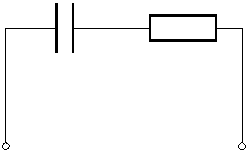
\includegraphics[]{chems/chem1}
	\caption{Последовательная $RC$ -- цепочка}
	\label{fig:RC}
\end{figure}

\subsubsection{Импеданс}
    
Импеданс $RC$ -- цепочки найдем, используя ранее вычисленные 
импедансы линейных элементов:
\begin{equation}
	\hat{z}=\frac{1}{i\cdot\omega C}+R
\end{equation}
\begin{equation}
	z=\sqrt{
		\frac{1}{\omega^2 C^2}	
		+R^2
	}=
	\sqrt{
		\frac{1}{\omega^2 C^2}	
		+\frac{R^2\omega^2 C^2}{\omega^2 C^2}
	}=\frac{\sqrt{1+(\omega RC)^2}}{\omega C}
\end{equation}
Экспериментально можно снимать зависомость $U_{13}\equiv U_\text{вх}$ и $U_{23}\equiv U_\text{вых}$ от частоты. Из закона Ома найдем тогда импеданс цепочки.
\begin{gather}
	\hat{J}_{13}=\hat{J}_{23} \quad\Rightarrow\quad
	\frac{\hat{U}_{13}}{\hat{z}}=\frac{\hat{U}_{23}}{R}
\end{gather}
Взяв по модулю, получим нужное соотношение:
\begin{equation}
	z=\frac{U_\text{вх}}{U_\text{вых}}R
\end{equation}

\subsubsection{Разность фаз}
Также найдем зависимость разности фаз от частоты:
\begin{equation}
	|\tan\phi| = |\frac{\Im\hat{z}}{\Re\hat{z}}|=
	|\frac{
		-(\omega C)^{-1}
	}{
		R
	}|=
	\frac{
		1
	}{
		\omega RC
	}	
\end{equation}

\subsubsection{Результаты эксперимента}
%!TEX root=../polypole.tex
\begin{table}[H]
	    \caption{Результаты эксперимента для первой схемы}
	    \label{tab:chem1}
	    \pgfkeys{/pgf/number format/.cd,
		fixed,  1000 sep={\,}}
\newlength\Colsep
\setlength\Colsep{10pt}
% \xdef\Table{data/i.tsv}
	     \xdef\C{5e-8}
\xdef\R{13000}  
\pgfplotstableset{
	% multicolumn names, % allows to have multicolumn names
	% header=has colnames,
	dec sep align,
	col sep=tab, % the seperator in our .csv file
	fixed zerofill, 
	precision=4,
    create on use/omega/.style={
        create col/expr={
        \thisrow{Fr}*2*3.14
        }
    },	 
    create on use/z/.style={
        create col/expr={
        13000*\thisrow{Uin}/\thisrow{Uout}
        }
    },				
	columns/z/.style={
		column name={$z$, Ом},
		precision=0		
	},	
	columns/Fr/.style={
		column name={$\nu$, Гц},
		precision=0,		
	},		
	columns/omega/.style={
		column name={$\omega$, Гц},
		precision=0,		
	},	
	columns/a/.style={
		column name={$a$},
		precision=1,		
	},		
	columns/b/.style={
		column name={$b$},
		precision=1,		
	},					
	columns/Uin/.style={
		column name={$U_{in}$, В},
		precision=3,		
		% column type/.add={|}{},
	},
	columns/Uout/.style={
		column name={$U_{in}$, В},
		precision=3,				
		% column type/.add={|}{},
	},
	columns/phi/.style={
		column name={$\phi$, рад},
		precision=2,				
		% column type/.add={|}{},
	},
	columns/dphi/.style={
		column name={$\Delta\phi$, рад},
		precision=2,				
		% column type/.add={|}{},
	},	
	columns/tanphi/.style={
		column name={$\tan\phi$},
		precision=3,				
		% column type/.add={|}{},
	},		
	empty cells with={\textbf{--}},
	every head row/.style={
	before row={\toprule},
	after row={
		\midrule}
		},
	every last row/.style={after row=\bottomrule},
	every row/.style={after row=\midrule}, 
	columns={Fr,omega,a,b,phi,tanphi,Uin,Uout,z},		
	% dec zerofill
	% fixed,fixed zerofill,
	% precision=3
	% every even column/.style={
	% 	% column type/.add={>{\columncolor[gray]{.8}}}{}
	% },
	% every even row/.style={
	% 	before row={\rowcolor[gray]{0.95}}
	% },	
	}
	\centering
	\pgfplotstabletypeset[]{data/chem1.tsv}

\end{table}
\begin{figure}[H]
	\centering
	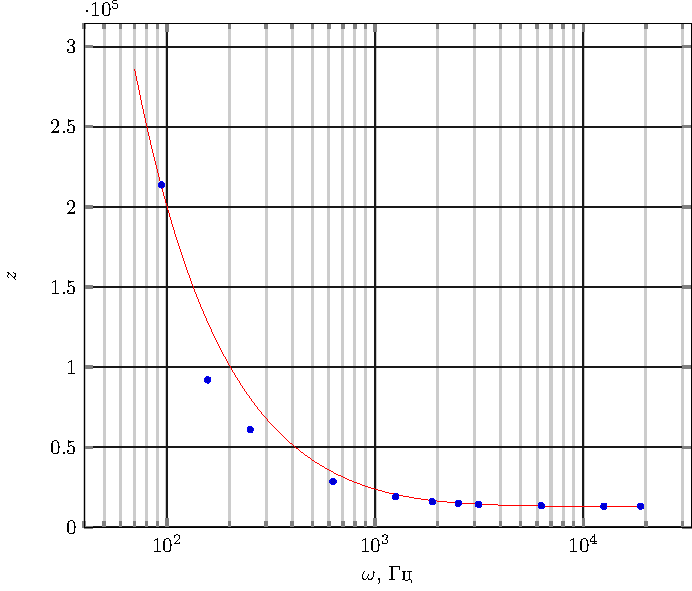
\includegraphics[width=0.85\textwidth]{img/chem1_z}
	\caption{Зависимость $z(\omega)$ для последовательной $RC$--цепочки}
	\label{fig:RC_z}
\end{figure}
\begin{figure}[H]
	\centering
	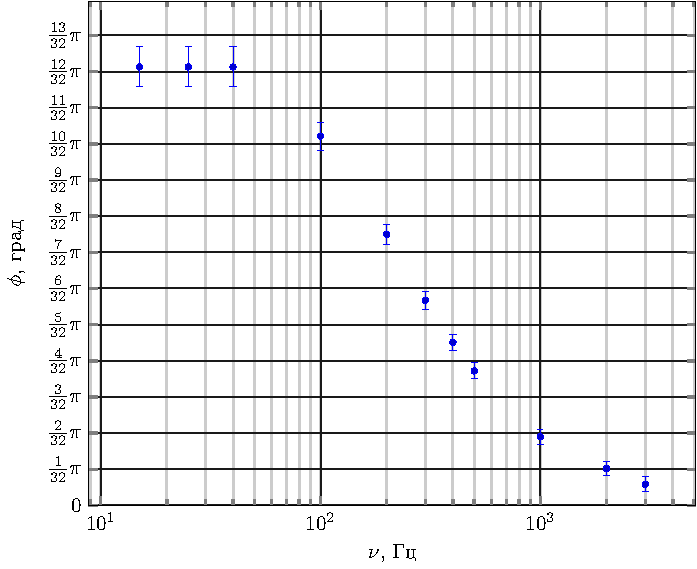
\includegraphics[width=0.85\textwidth]{img/chem1_phi} 
	\caption{Зависимость $\tan\phi(\omega)$ для последовательной $RC$--цепочки}
	\label{fig:RC_tanphi}
\end{figure}


\subsection{Схема №2. Последовательная $LC$ -- цепочка}
\begin{figure}[H]
	\centering
	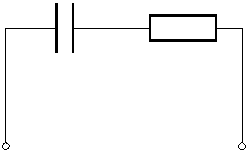
\includegraphics[]{chems/chem1}
	\caption{Последовательная $LC$ -- цепочка}
	\label{fig:LC}
\end{figure}

\subsubsection{Импеданс}
\begin{equation}
	\hat{z}=i\omega L+R
\end{equation}
\begin{equation}
	z=\sqrt{(\omega L)^2+R}
\end{equation}
Очевидно, что аналогично последовательной $RC$--цепочке
\begin{equation}
	z=\frac{U_\text{вх}}{U_\text{вых}}R
\end{equation}
\subsubsection{Разность фаз}
\begin{equation}
	\left|\tan\phi\right| = \left|\frac{\Im\hat{z}}{\Re\hat{z}}\right|=
	\left|\frac{
		\omega L
	}{
		R
	}\right|=
	\frac{
		\omega L
	}{
		R
	}	
\end{equation}

\subsubsection{Результаты эксперимента}

%!TEX root=../polypole.tex
\begin{table}[H]
	    \caption{Результаты эксперимента для второй схемы}
	    \label{tab:chem1}
	    \pgfkeys{/pgf/number format/.cd,
		fixed,  1000 sep={\,}}
% \xdef\Table{data/i.tsv}
	     \xdef\C{5e-8}
\xdef\R{13000}  
\pgfplotstableset{
	% multicolumn names, % allows to have multicolumn names
	% header=has colnames,
	dec sep align,
	col sep=tab, % the seperator in our .csv file
	fixed zerofill, 
	precision=4,
    create on use/omega/.style={
        create col/expr={
        \thisrow{Fr}*2*3.14
        }
    },	 
    create on use/z/.style={
        create col/expr={
        13000*\thisrow{Uin}/\thisrow{Uout}
        }
    },				
	columns/z/.style={
		column name={$z$, Ом},
		precision=0		
	},	
	columns/Fr/.style={
		column name={$\nu$, Гц},
		precision=0,		
	},		
	columns/omega/.style={
		column name={$\omega$, Гц},
		precision=0,		
	},	
	columns/a/.style={
		column name={$a$},
		precision=1,		
	},		
	columns/b/.style={
		column name={$b$},
		precision=1,		
	},					
	columns/Uin/.style={
		column name={$U_{in}$, В},
		precision=3,		
		% column type/.add={|}{},
	},
	columns/Uout/.style={
		column name={$U_{in}$, В},
		precision=3,				
		% column type/.add={|}{},
	},
	columns/phi/.style={
		column name={$\phi$, рад},
		precision=2,				
		% column type/.add={|}{},
	},
	columns/dphi/.style={
		column name={$\Delta\phi$, рад},
		precision=2,				
		% column type/.add={|}{},
	},	
	columns/tanphi/.style={
		column name={$\tan\phi$},
		precision=3,				
		% column type/.add={|}{},
	},		
	empty cells with={\textbf{--}},
	every head row/.style={
	before row={\toprule},
	after row={
		\midrule}
		},
	every last row/.style={after row=\bottomrule},
	every row/.style={after row=\midrule}, 
	columns={Fr,omega,a,b,phi,tanphi,Uin,Uout,z},		
	% dec zerofill
	% fixed,fixed zerofill,
	% precision=3
	% every even column/.style={
	% 	% column type/.add={>{\columncolor[gray]{.8}}}{}
	% },
	% every even row/.style={
	% 	before row={\rowcolor[gray]{0.95}}
	% },	
	}
	\centering
	\pgfplotstabletypeset[]{data/chem2.tsv}

\end{table}
\begin{figure}[H]
	\centering
	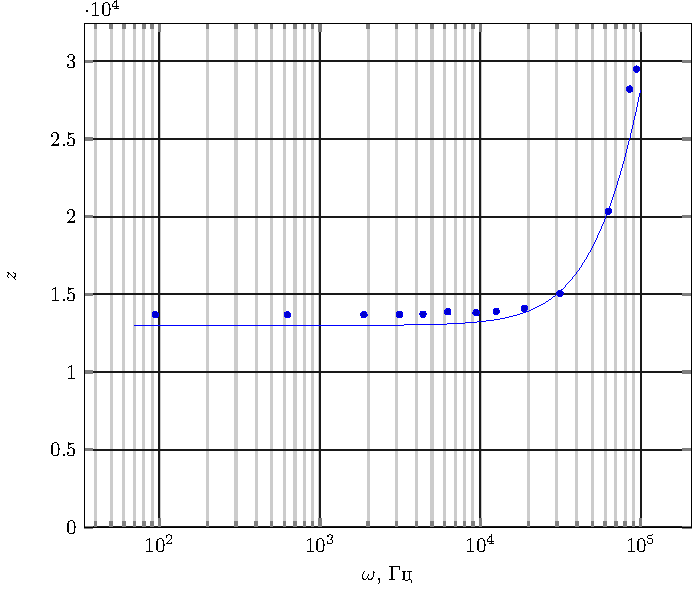
\includegraphics[width=0.85\textwidth]{img/chem2_z}
	\caption{Зависимость $z(\omega)$ для последовательной $LC$--цепочки}
	\label{fig:LC_z}
\end{figure}
\begin{figure}[H]
	\centering
	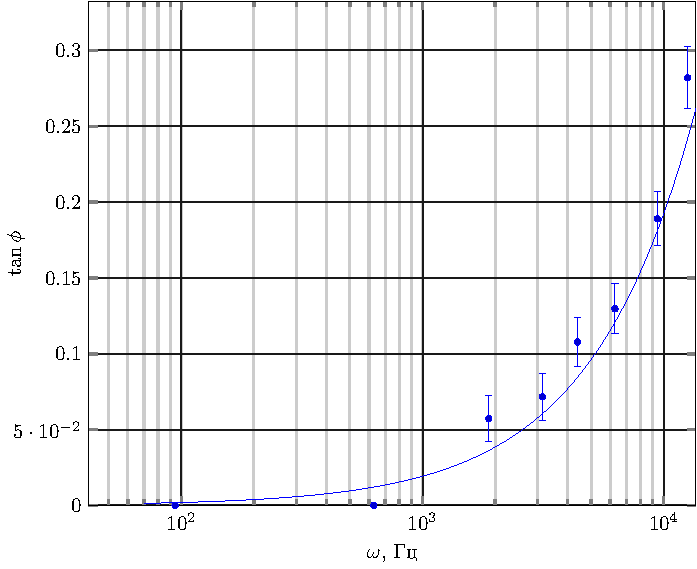
\includegraphics[width=0.85\textwidth]{img/chem2_phi} 
	\caption{Зависимость $\tan\phi(\omega)$ для последовательной $LC$--цепочки}
	\label{fig:LC_tanphi}
\end{figure}

\subsection{Схема №3. Двухполюсник $R[RC]$}
\begin{figure}[H]
	\centering
	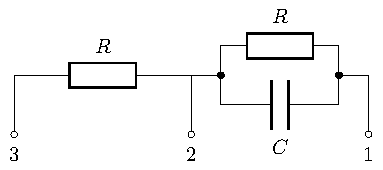
\includegraphics[]{chems/chem3}
	\caption{Двухполюсник $R[RC]$}
	\label{fig:RRC}
\end{figure}

\subsubsection{Импеданс}
Сначала рассчитаем импеданс параллельно соединенных конденсатора и резистора $R$
\begin{equation}
	\frac{1}{\hat{z}_0}=\frac{1}{R}+i\omega C
\end{equation}
\begin{equation}
	\hat{z}_0=\frac{R}{1+i \omega CR}
\end{equation}
Комплексный импеданс всей схемы будет равен:
\begin{equation}
	\hat{z}=\hat{z}_0+R=\frac{R}{1+i \omega RC}+R=
	\frac{R(1-i \omega RC)}{1+(\omega RC)^2}+R
\end{equation}
\begin{equation}
	z=\sqrt{\Im^2\hat{z}+\Re^2\hat{z}}=
	R\sqrt{
	\left(
	1+\frac{1}{1+(\omega RC)^2}
	\right)^2+
	\left(
	\frac{\omega C}{1+(\omega RC)^2}
	\right)^2
	}
\end{equation}

\subsubsection{Разность фаз}
\begin{equation}
	\tan\phi = \frac{\Im\hat{z}}{\Re\hat{z}}=
	\frac{
		-\frac{\omega R^2C}{1+(\omega RC)^2}
	}{
		\frac{R+R+R(\omega RC)^2}{1+(\omega RC)^2}
	}=
	\frac{
		-\omega R^2C
	}{
		R+R+R(\omega RC)^2
	}=
	-\frac{
		\omega RC
	}{
		2+(\omega RC)^2
	}	
\end{equation}
Из уравнения видно, что на малых частотах $z\approx 2R$, а при высоких $z\approx R$.

\subsubsection{Результаты эксперимента}

%!TEX root=../polypole.tex
\begin{table}[H]
	    \caption{Результаты эксперимента для третей схемы}
	    \label{tab:chem1}
	    \pgfkeys{/pgf/number format/.cd,
		fixed,  1000 sep={\,}}
% \xdef\Table{data/i.tsv}
	     \xdef\C{5e-8}
\xdef\R{13000}  
\pgfplotstableset{
	% multicolumn names, % allows to have multicolumn names
	% header=has colnames,
	dec sep align,
	col sep=tab, % the seperator in our .csv file
	fixed zerofill, 
	precision=4,
    create on use/omega/.style={
        create col/expr={
        \thisrow{Fr}*2*3.14
        }
    },	 
    create on use/z/.style={
        create col/expr={
        13000*\thisrow{Uin}/\thisrow{Uout}
        }
    },				
	columns/z/.style={
		column name={$z$, Ом},
		precision=0		
	},	
	columns/Fr/.style={
		column name={$\nu$, Гц},
		precision=0,		
	},		
	columns/omega/.style={
		column name={$\omega$, Гц},
		precision=0,		
	},	
	columns/a/.style={
		column name={$a$},
		precision=1,		
	},		
	columns/b/.style={
		column name={$b$},
		precision=1,		
	},					
	columns/Uin/.style={
		column name={$U_{in}$, В},
		precision=3,		
		% column type/.add={|}{},
	},
	columns/Uout/.style={
		column name={$U_{in}$, В},
		precision=3,				
		% column type/.add={|}{},
	},
	columns/phi/.style={
		column name={$\phi$, рад},
		precision=2,				
		% column type/.add={|}{},
	},
	columns/dphi/.style={
		column name={$\Delta\phi$, рад},
		precision=2,				
		% column type/.add={|}{},
	},	
	columns/tanphi/.style={
		column name={$\tan\phi$},
		precision=3,				
		% column type/.add={|}{},
	},		
	empty cells with={\textbf{--}},
	every head row/.style={
	before row={\toprule},
	after row={
		\midrule}
		},
	every last row/.style={after row=\bottomrule},
	every row/.style={after row=\midrule}, 
	columns={Fr,omega,a,b,phi,tanphi,Uin,Uout,z},		
	% dec zerofill
	% fixed,fixed zerofill,
	% precision=3
	% every even column/.style={
	% 	% column type/.add={>{\columncolor[gray]{.8}}}{}
	% },
	% every even row/.style={
	% 	before row={\rowcolor[gray]{0.95}}
	% },	
	}
	\centering
	\pgfplotstabletypeset[]{data/chem3.tsv}

\end{table}
\begin{figure}[H]
	\centering
	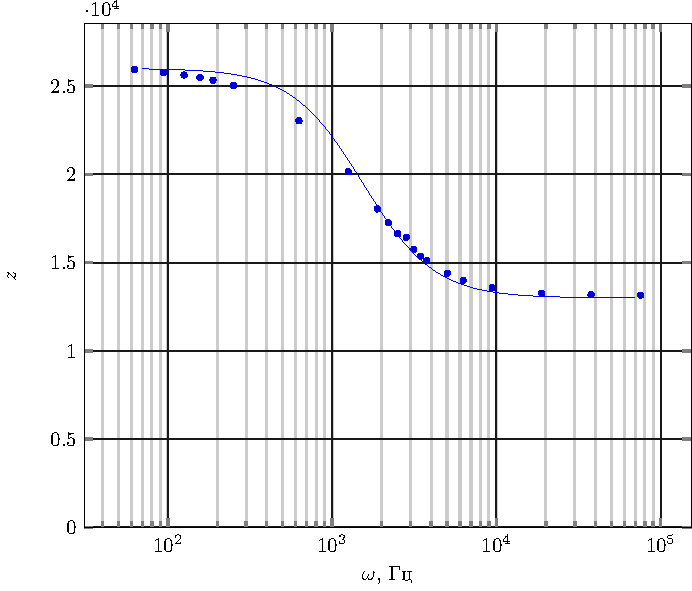
\includegraphics[width=0.85\textwidth]{img/chem3_z}
	\caption{Зависимость $z(\omega)$ для  $R[RC]$--двухполюсника}
	\label{fig:RRC_z}
\end{figure}
\begin{figure}[H]
	\centering
	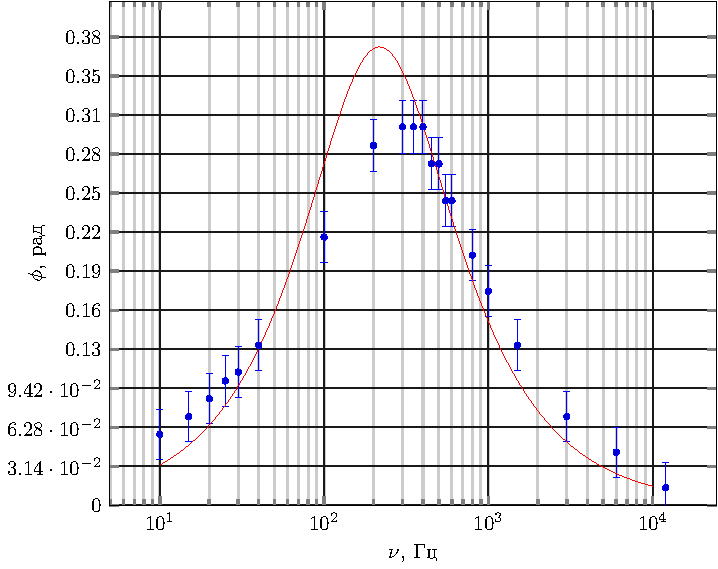
\includegraphics[width=0.85\textwidth]{img/chem3_phi} 
	\caption{Зависимость $\tan\phi(\omega)$ для $R[RC]$--двухполюсника}
	\label{fig:RRC_tanphi}
\end{figure}


\subsection{Схема №4. Двухполюсник $R[RL]$}
\begin{figure}[H]
	\centering
	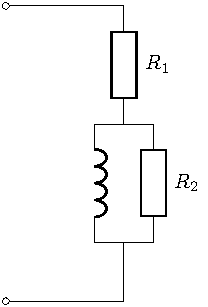
\includegraphics[]{chems/chem4}
	\caption{Двухполюсник $R[RL]$}
	\label{fig:RRL}
\end{figure}
\subsubsection{Импеданс}
Рассчитаем импеданс параллельно соединенных катушки и резистора $R$
\begin{equation}
	\frac{1}{\hat{z_0}}=\frac{1}{R}+\frac{1}{i\omega L}=\frac{R+i\omega L}{iR\omega L}=\frac{\omega L - iR}{\omega R L}
\end{equation}
\begin{equation}
	\hat{z_0}=\frac{\omega R L(\omega L + iR)}{(\omega L - iR)(\omega L + iR)}=
	\frac{\omega^2L^2 R +i\omega L R^2}{\omega^2L^2+R^2}
\end{equation}
А импеданс всей схемы:
\begin{equation}
	\hat{z}=
	\left(
	\frac{2\omega^2L^2 R+R^3}{\omega^2L^2+R^2}
	\right)+
	i
	\left(
	\frac{\omega L R^2}{\omega^2L^2+R^2}
	\right)
\end{equation}
\begin{equation}
	z=\sqrt{\Im^2\hat{z}+\Re^2\hat{z}}=
	\frac{1}{\omega^2L^2+R^2}\sqrt{
	\left(
	2\omega^2L^2 R+R^3
	\right)^2+
	\left(
	\omega L R^2
	\right)^2
	}
\end{equation}
При больших частотах можно пренебречь вторым слагаемым под корнем и сопротивлением в суммах, тогда видно, что на таких частотах $z\approx 2R$.

На малых частотах $\omega\approx0$ предел даёт значение импеданса $R$.
\subsubsection{Разность фаз}
\begin{equation}
	\tan\phi = \frac{\Im\hat{z}}{\Re\hat{z}}=
	\frac{
		\omega L R^2
	}{
		2\omega^2L^2 R+R^3
	}=
	\frac{
		\omega LR
	}{
		2\omega^2L^2 +R^2
	}	
\end{equation}

\subsubsection{Результаты эксперимента}

%!TEX root=../polypole.tex
\begin{table}[H]
	    \caption{Результаты эксперимента для четвёртой схемы}
	    \label{tab:chem1}
	    \pgfkeys{/pgf/number format/.cd,
		fixed,  1000 sep={\,}}
% \xdef\Table{data/i.tsv}
	     \xdef\C{5e-8}
\xdef\R{13000}  
\pgfplotstableset{
	% multicolumn names, % allows to have multicolumn names
	% header=has colnames,
	dec sep align,
	col sep=tab, % the seperator in our .csv file
	fixed zerofill, 
	precision=4,
    create on use/omega/.style={
        create col/expr={
        \thisrow{Fr}*2*3.14
        }
    },	 
    create on use/z/.style={
        create col/expr={
        13000*\thisrow{Uin}/\thisrow{Uout}
        }
    },				
	columns/z/.style={
		column name={$z$, Ом},
		precision=0		
	},	
	columns/Fr/.style={
		column name={$\nu$, Гц},
		precision=0,		
	},		
	columns/omega/.style={
		column name={$\omega$, Гц},
		precision=0,		
	},	
	columns/a/.style={
		column name={$a$},
		precision=1,		
	},		
	columns/b/.style={
		column name={$b$},
		precision=1,		
	},					
	columns/Uin/.style={
		column name={$U_{in}$, В},
		precision=3,		
		% column type/.add={|}{},
	},
	columns/Uout/.style={
		column name={$U_{out}$, В},
		precision=3,				
		% column type/.add={|}{},
	},
	columns/phi/.style={
		column name={$\phi$, рад},
		precision=2,				
		% column type/.add={|}{},
	},
	columns/dphi/.style={
		column name={$\Delta\phi$, рад},
		precision=2,				
		% column type/.add={|}{},
	},	
	columns/tanphi/.style={
		column name={$\tan\phi$},
		precision=3,				
		% column type/.add={|}{},
	},		
	empty cells with={\textbf{--}},
	every head row/.style={
	before row={\toprule},
	after row={
		\midrule}
		},
	every last row/.style={after row=\bottomrule},
	every row/.style={after row=\midrule}, 
	columns={Fr,omega,a,b,phi,tanphi,Uin,Uout,z},		
	% dec zerofill
	% fixed,fixed zerofill,
	% precision=3
	% every even column/.style={
	% 	% column type/.add={>{\columncolor[gray]{.8}}}{}
	% },
	% every even row/.style={
	% 	before row={\rowcolor[gray]{0.95}}
	% },	
	}
	\centering
	\pgfplotstabletypeset[]{data/chem4.tsv}

\end{table}
\begin{figure}[H]
	\centering
	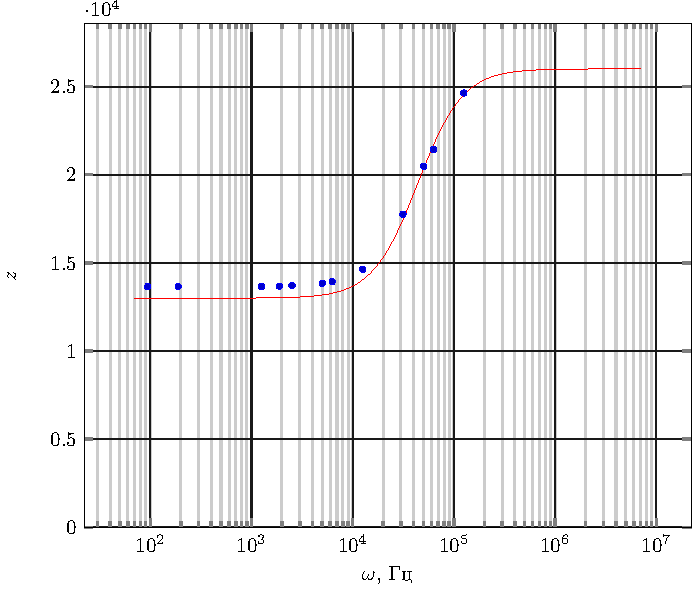
\includegraphics[width=0.85\textwidth]{img/chem4_z}
	\caption{Зависимость $z(\omega)$ для  $R[RL]$--двухполюсника}
	\label{fig:RRL_z}
\end{figure}
\begin{figure}[H]
	\centering
	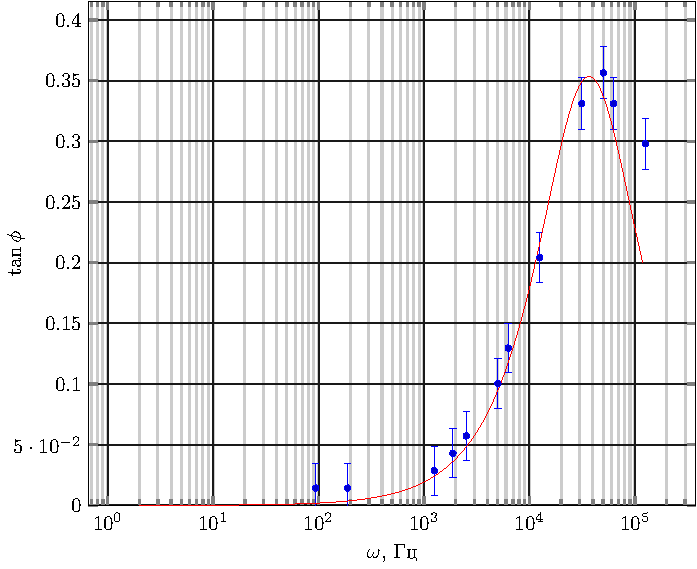
\includegraphics[width=0.85\textwidth]{img/chem4_phi} 
	\caption{Зависимость $\tan\phi(\omega)$ для $R[RL]$--двухполюсника}
	\label{fig:RRL_tanphi}
\end{figure}


\section{Четырехполюсники. Расчет цепи и экспериментальные данные}

\subsection{Схема №5. Простейший мостовой фазовращатель}

\begin{figure}[H]
	\centering
	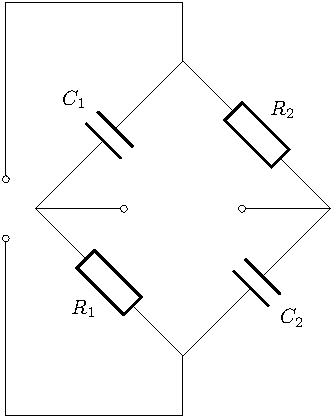
\includegraphics[]{chems/chem5}
	\caption{Принципиальная схема фазовращателя}
	\label{fig:ph_rot}
\end{figure}

Запишем ток через левую ветвь:
\begin{equation}
	\hat{J}_{left}\equiv \hat{J}_{R_1}=\frac{\hat{U}_{in}}{R_1+\frac{1}{i\omega C_1}}
\end{equation}
Аналогично через правую:
\begin{equation}
	\hat{J}_{right}\equiv \hat{J}_{R_2}=\frac{\hat{U}_{in}}{R_2+\frac{1}{i\omega C_2}}
\end{equation}
Тогда 
\begin{equation}
	\hat{U}_{out}\equiv\hat{U}_{MN}=
	-\hat{U}_{AM}+\hat{U}_{AN}=
	-\hat{J}_{left}\cdot\frac{1}{i\omega C_1}
	+\hat{J}_{right}\cdot R_2
\end{equation}
\begin{equation}
	\hat{U}_{out}=\hat{U}_{in}
	\left(
	\frac{R_2}{R_2+(i\omega C_2)^{-1}}-
	\frac{1}{i\omega C_1}\frac{1}{R_1+(i\omega C_1)^{-1}}
	\right)
\end{equation}
\begin{equation}
	\hat{K}=\frac{\hat{U}_{out}}{\hat{U}_{in}}=
	\frac{i\omega C_2 R_2}{i\omega C_2 R_2+1}-
	\frac{1}{i\omega C_1 R_1+1}
\end{equation}
Обозначим $\Omega_1=\omega C_1R_1$, $\Omega_2=\omega C_2R_2$:
\begin{equation}
	\hat{K}=\frac{i\Omega_2}{i\Omega_2+1}-\frac{1}{i\Omega_1+1}=
	\frac{i\Omega_2(1-i\Omega_2)}{\Omega_2^2+1}+\frac{i\Omega_1-1}{\Omega_1^2+1}
\end{equation}
\begin{equation}
	\hat{K}=
	\left(
		\frac{\Omega_2^2}{\Omega_2^2+1}-
		\frac{1}{\Omega_1^2+1}
	\right)+
	i\left(
		\frac{\Omega_2}{\Omega_2^2+1}+
		\frac{\Omega_1}{\Omega_1^2+1}
	\right)
\end{equation}
Отсюда
\begin{equation}
	K=
	\sqrt{
	\left(
		\frac{\Omega_2^2}{\Omega_2^2+1}-
		\frac{1}{\Omega_1^2+1}
	\right)^2+
	\left(
		\frac{\Omega_2}{\Omega_2^2+1}+
		\frac{\Omega_1}{\Omega_1^2+1}
	\right)^2
	}
\end{equation}
При $\Omega_1$=$\Omega_2$ подстановка дает $K\equiv 1$.

\begin{equation}
	\tan\phi=\left(
		\frac{\Omega_2}{\Omega_2^2+1}+
		\frac{\Omega_1}{\Omega_1^2+1}
	\right)
	\cdot
	\left(
		\frac{\Omega_2^2}{\Omega_2^2+1}-
		\frac{1}{\Omega_1^2+1}
	\right)^{-1}
\end{equation}
При $\Omega_1$=$\Omega_2 \equiv \Omega$
\begin{equation}
	\tan\phi=\frac{2\Omega}{1-\Omega^2}
\end{equation}
Можно заметить, что это формула тангенса половинного угла:
\begin{equation}
	\tan\phi=\frac{2\tan\frac{\phi}{2}}{1-\tan^2\frac{\phi}{2}}
\end{equation}

Отсюда
\begin{equation}
	\tan\frac{\phi}{2}=\Omega = \omega RC
\end{equation}

Так как $\arctan\Omega$ может принимать значения только от 0 до $\frac{\pi}2$, то 
\begin{equation}
	0\leq\phi<\pi
\end{equation}

\subsection{Схема №6. Составной четырехполюсник - фазовращатель}

\begin{figure}[H]
	\centering
	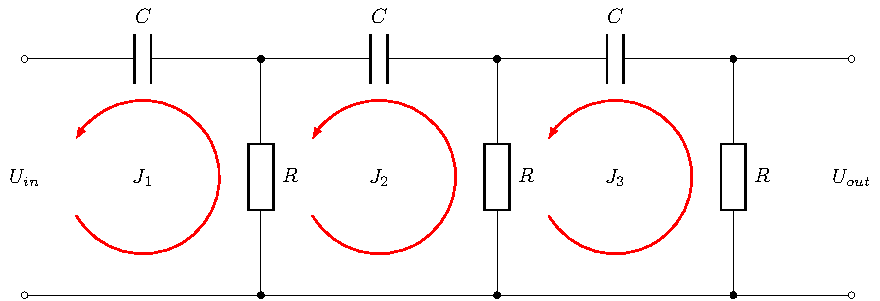
\includegraphics[]{chems/chem6}
	\caption{Принципиальная схема фазовращателя}
	\label{fig:ph_rot2}
\end{figure}

\subsubsection{Расчет комплексного коэффициента передачи}

Рассчитаем цепь четырехполюсника с помощью метода контурных токов. Уравнения будут выглядеть следующим образом:
\begin{gather}
	\left\{
	\begin{aligned}
		J_1\cdot\left(\frac{1}{i\omega C}+R\right)+J_2\cdot\left( -R \right)+J_3\cdot\left(0 \right)=U_{in}\\
		J_1\cdot\left(-R\right)+J_2\cdot\left( \frac{1}{i\omega C}+2R \right)+J_3\cdot\left(-R \right)=0\\
		J_1\cdot\left(0\right)+J_2\cdot\left( -R \right)+J_3\cdot\left(\frac{1}{i\omega C}+2R \right)=0
	\end{aligned}
	\right.
\end{gather}
В этом расчете все величины -- комплексные, хотя это явно не указано. Методом Крамера найдем $J_3$:
\begin{equation}
\Delta =\begin{vmatrix} 
		\alpha & -R & 0\\
		-R & \alpha+R & -R\\
		0 & -R & \alpha+R\\
	\end{vmatrix}=
\alpha[(\alpha+R)^2-R^2]+R[-R(\alpha+R)]
\end{equation}
\begin{equation}
\Delta_3 =\begin{vmatrix} 
		\alpha & -R & U_{in}\\
		-R & \alpha+R & 0\\
		0 & -R & 0\\
	\end{vmatrix}=
R^2U_{in}
\end{equation}
Здесь $\alpha=\cfrac{1}{i\omega C}+R$. Тогда
\begin{multline}
	-\Delta=R^3+R^2\alpha-\alpha^3-2\alpha^2R=
	R^3
	+R^2\frac{1}{i\omega C}
	+R^3
	-\frac{i}{\omega^3C^3}
	+3R\frac{1}{\omega^2C^2}
	-3R^2\frac{i}{i\omega C}
	-\\-R^3
	+2R\frac{1}{\omega^2C^2}
	-4R^2\frac{1}{i\omega C}
	-2R^3
	=\\=
	5R\frac{1}{\omega^2C^2}
	-6R^2\frac{1}{i\omega C}
	-R^3
	-\frac{i}{\omega^3 C^3}	
\end{multline}
\begin{equation}
	\Delta=
	\left(
	R^3
	-\frac{5R}{\omega^2C^2}
	\right)
	+i
	\left(
	\frac{1}{\omega^3C^3}
	-\frac{6R^2}{\omega C}
	\right)	
\end{equation}
Или поделив на $R^3$ и обозначив $\Omega=\omega RC$
\begin{equation}
	\cfrac{\Delta}{R^3}=
	\left(
	1
	-\frac{5}{\Omega^2}
	\right)
	+i
	\left(
	\frac{1}{\Omega^3}
	-\frac{6}{\Omega}
	\right)=a+ib
\end{equation}

\begin{equation}
	\label{eq:imre}
	K=\frac{U_{out}}{U_{in}}=R\frac{J_3}{U_{in}}=\frac{R}{U_{in}}\frac{\Delta_3}{\Delta}=\frac{R^3}{\Delta}=\frac{1}{a+ib}=\frac{a-ib}{a^2+b^2}
\end{equation}
Отсюда, очевидно, модуль амплитудной характеристики
\begin{equation}
	|K|=\frac{1}{|a+ib|}=\frac{1}{\sqrt{a^2+b^2}}
	=
	\cfrac{1}{
	\sqrt{
	\left(
		1
		-\cfrac{5}{\Omega^2}
	\right)^2
	+
	\left(
		\cfrac{1}{\Omega^3}
		-\cfrac{6}{\Omega}
	\right)^2	
	}}
\end{equation}
Упростим, домножив на $\Omega^3$ числитель и знаменатель:
\begin{equation}
	|K|=
	\cfrac{\Omega^3}{
	\sqrt{
	\Omega^2\left(
		5-\Omega^2
	\right)^2
	+
	\left(
		1
		-{6}{\Omega}^2
	\right)^2	
	}}
\end{equation}
Из (\ref{eq:imre}), очевидно,
\begin{equation}
	\tan\phi=-\frac{b}{a}=-\frac{1-6\Omega^2}{\Omega(5-\Omega^2)}
\end{equation}
\begin{equation}
	\phi=\arctan
	\left(
		-\frac{1-6\Omega^2}{\Omega(5-\Omega^2)}
	\right)
\end{equation}
Воспользуемся тригонометрической формулой
\begin{equation}
	\arctan x = \frac{\pi}{2}-\arctan\frac{1}{x}
\end{equation}
\begin{equation}
	\phi=\frac{\pi}{2}-\arctan(-\frac{\Omega(5-\Omega^2)}{1-6\Omega^2})
\end{equation}
\begin{equation}
	\phi=\frac{\pi}{2}+\arctan\frac{\Omega(5-\Omega^2)}{1-6\Omega^2}
\end{equation}

\subsubsection{Расчет импеданса входа}
    
\begin{equation}
	z=\frac{1}{i\omega C}+
	\cfrac{1}{
		\cfrac{1}{R}+
		\cfrac{1}{
			\cfrac{1}{i\omega C}+
			\cfrac{1}{
				\frac{1}{R}+
					\cfrac{1}{
						R+
						\cfrac{1}{
							i\omega C				
						}
					}
				}
			}		
			}=
\frac{1}{i\omega C}+
	\cfrac{1}{
		\cfrac{1}{R}+
		\cfrac{1}{
			\cfrac{1}{i\omega C}+
			\cfrac{1}{
				\frac{1}{R}+
					\cfrac{i\omega C}{i\Omega+1}
				}
			}		
			}
\end{equation}
\begin{gather}
=
\frac{1}{i\omega C}+
	\cfrac{1}{
		\cfrac{1}{R}+
		\cfrac{1}{
			\cfrac{1}{i\omega C}+
			\cfrac{R(i\Omega+1)}{2i\Omega+1}	
		}	
	}
=\\=
\frac{1}{i\omega C}+
	\cfrac{1}{
		\cfrac{1}{R}+		
			\cfrac{i\omega C - 2\Omega \omega C}{3i\Omega-\Omega^2}
	}
=\\=
\frac{1}{i\omega C}+
	\cfrac{1}{
		\cfrac{3i\Omega-\Omega^2}{...}+		
			\cfrac{i\Omega - 2\Omega^2}{R(3i\Omega-\Omega^2)}
	}
=\\=
\frac{1}{i\omega C}+
\cfrac{R(3i\Omega-\Omega^2)}{4i\Omega - 3\Omega^2}
=\\=
\frac{4i\Omega - 3\Omega^2}{...}+
\cfrac{i\Omega(3i\Omega-\Omega^2)}{-4\Omega\omega C - 3i\Omega^2\omega C}
=\\=
\frac{4i\Omega - 3\Omega^2}{...}+
\cfrac{-3\Omega^2-i\Omega^3}{-4\Omega\omega C - 3i\Omega^2\omega C}
=\\=
R\frac{
	i\Omega^3
	+6\Omega^2
	-4i\Omega 
}{
	4\Omega^2 
	+3i\Omega^3
}
=\\=
R\frac{
	(i\Omega^3
	+6\Omega^2
	-4i\Omega )
	(
		4\Omega^2 
		-3i\Omega^3	
	)
}{
	16\Omega^4
	+9\Omega^6
}
=R\frac{
	-16 i \Omega^3 + 12 \Omega^4 - 14 i \Omega^5 + 3 \Omega^6
}{
	16\Omega^4
	+9\Omega^6
}
=\\=
\left(
R
	\frac{
		12 \Omega^4 + 3 \Omega^6
	}{
		16\Omega^4
		+9\Omega^6
	}
\right)
-i
\left(
	R\frac{
		16 \Omega^3 + 14 \Omega^5
	}{
		16\Omega^4
		+9\Omega^6
	}
\right)
\end{gather}

\section{Схема с рисунка 5}
\begin{center}
\documentclass[border=1pt]{standalone}
\usepackage[europeanresistors,americaninductors]{circuitikz}
\usepackage{amssymb}
\begin{document}
\begin{circuitikz}[]
	\draw (0,0) coordinate(0) to [short,o-*] (2,0) coordinate (1)
	to (2,1) 
	to [R,R=$R$] (4,1)
	to [L,L=$L$] (6,1)
	to (6,0) coordinate(2)
	to [short,*-*](7,0) coordinate(3)
	to [short,-o](9,0) coordinate (0');
	\draw (1) to ++ (0,-1)
	to [R,R=$R$]++ (2,0)
	to [C=$C$]++ (2,0)
	to (2)
	;
	\draw (3) to [short,*-*,R=$R$] ++ (0,-3)
	;
	\draw  (0,-3) to [short,o-o] (9,-3) ;
	\draw (0,-1.5) node[below] {$U_{in}$};
	\draw (9,-1.5) node[below] {$U_{out}$};
	

\end{circuitikz}
\end{document}
\end{center}

Сначала рассчитаем импеданс парралельно соединенных RL и RC контуров.
\begin{equation}
	\frac{1}{\hat{z_0}}=\frac{1}{\hat{z_1}}+\frac{1}{\hat{z_2}}=\frac{1}{R+i\omega L}+\frac{i\omega C}{iR\omega C+1}
\end{equation}
\begin{equation}
\frac{1}{\hat{z_0}}=\frac{1-\omega^2 CL+i2R\omega C}{R(1-\omega^2 LC)+i\omega(R^2C+L)}
\end{equation}
Учитывая то, что $L=\kappa R$ и $C=\frac{\kappa}{R}$ получим
\begin{equation}
	\hat{z_0}=\frac{R-\omega^2\kappa L+i\omega R\kappa +i\omega \kappa R}{1-\omega^2\kappa RC+i2\omega\kappa}
\end{equation}
Отсюда следует, что
\begin{equation}
	\hat{z_0}=R
\end{equation}
Получается, что данная цепь ни что иное как потенциометр. 
\begin{equation}
	K_U=\frac{R}{R+R}=\frac{1}{2}
\end{equation}

\section{Схема с рисунка 6}
\begin{center}
\documentclass[border=1pt]{standalone}
\usepackage[europeanresistors,americaninductors]{circuitikz}
\usepackage{amssymb}
\begin{document}
\begin{circuitikz}[]
	\draw (0,0) coordinate(0) to [short,o-*] (1,0) coordinate (1)
	to [R=$2R$]++ (3,0) coordinate(5)
	to [short,*-*,R=$2R$]++ (3,0) 
	to [short,*-o]++ (1,0);
	\draw (1) to [C=$C$] ++ (0,-2)
	to ++ (1.5,0) coordinate(3)
	to (7,-2)
	to [C=$C$] ++ (0,2);
	\draw (3) to [short,-*,R=$R$] ++ (0,-2)
	to [short,-o]++ (-2.5,0)
	to [short,-*](4,-4) coordinate (4)
	to [] ++ (1.5,0)
	to [short,-o](8,-4);
 	\draw (4) to ++(0,2)
 	to [C=$2C$]++(0,2);

 	\draw (8,-2) node[right] {$U_{out}$};
 	\draw (0,-2) node[left] {$U_{in}$};
	\end{circuitikz}
\end{document}
\end{center}
Перейдём к эквивалентной схеме:
\begin{center}
\documentclass[border=1pt]{standalone}
\usepackage[europeanresistors,americaninductors]{circuitikz}
\usepackage{amssymb}
\begin{document}
\begin{circuitikz}[]
\draw (0,0) to [short,o-,R=$2R$] (8,0)
	to (8,-2)
	to [C=$2C$] (8,-4)
	to [short,-o](0,-4);
\draw (1,0) to [short,*-*,C=$C$](1,-2) coordinate(1)
	to (1,-2) to [short,-*,R=$R$](1,-4);
\draw	(1) to [C=$C$] ++ (3,0)
	to [short,-*,R=$2R$] ++ (4,0);
\draw (4,-2) to [short,-o]++ (0,-0.75);
\draw (4,-4) to [short,-o]++ (0,0.75);
\draw (4,-3) node [right] {$U_{out}$};
\draw (0,-2) node [left] {$U_{in}$};
	\end{circuitikz}
\end{document}
\end{center}

$U_{out}=U_{2R}+U_{2C}$


$U_{2R}=(J_3-J_2)\cdot 2R$


$U_{2C}=J_3\cdot\frac{1}{2i\omega C}$  

Все величины подразумеваются комплексными.

 Методом контурных токов составим систему уравнений:
\begin{gather}
	\left\{
	\begin{aligned}
		J_1\cdot\left(\frac{1}{i\omega C}+R\right)+J_2\cdot\left( -\frac{1}{i\omega C} \right)+J_3\cdot\left(R \right)=U_{in}\\
		J_1\cdot\left(-\frac{1}{i\omega C}\right)+J_2\cdot\left(4R+\frac{2}{i\omega C} \right)+J_3\cdot\left(-2R-\frac{1}{i\omega C} \right)=0\\
		J_1\cdot\left(-R\right)+J_2\cdot\left( -2R-\frac{1}{i\omega C} \right)+J_3\cdot\left(\frac{3}{2i\omega C}+3R \right)=0
	\end{aligned}
	\right.
\end{gather}
Решим её методом Краммера:
\begin{equation}
	\Delta =\begin{vmatrix} 
		R+\frac{1}{i\omega C} & -\frac{1}{i\omega C} & -R\\
		-\frac{1}{i\omega C} & 4R+\frac{2}{i\omega C} & -2R-\frac{1}{i\omega C}\\
		-R & -\frac{1}{i\omega C}-2R & 3R+\frac{3}{2i\omega C}\
	\end{vmatrix}=
\frac{(2i\omega CR+1)[4(i\omega CR)^2+8(i\omega CR)+1]}{2(i\omega C)^3}
\end{equation}
\begin{equation}
	\Delta_{J_1} =\begin{vmatrix} 
		U_{in} & -\frac{1}{i\omega C} & -R\\
		0 & 4R+\frac{2}{i\omega C} & -2R-\frac{1}{i\omega C}\\
		0 & -\frac{1}{i\omega C}-2R & 3R+\frac{3}{2i\omega C}\
	\end{vmatrix}=
\frac{2U_{in}(2i\omega CR+1)^2}{(i\omega C)^2}	
\end{equation}
\begin{equation}
	\Delta_{J_2} =\begin{vmatrix} 
		R+\frac{1}{i\omega C} & U_{in} & -R\\
		-\frac{1}{i\omega C} & 0 & -2R-\frac{1}{i\omega C}\\
		-R & 0 & 3R+\frac{3}{2i\omega C}\
	\end{vmatrix}=
		\frac{U_{in}(2i\omega CR+1)(2i\omega CR+3)}{(i\omega C)^2}	
\end{equation}
\begin{equation}
	\Delta_{J_3} =\begin{vmatrix} 
		R+\frac{1}{i\omega C} & -\frac{1}{i\omega C} & U_{in}\\
		-\frac{1}{i\omega C} & 4R+\frac{2}{i\omega C} & 0\\
		-R & -\frac{1}{i\omega C}-2R & 0\
	\end{vmatrix}=
	\frac{U_{in}(2i\omega CR+1)^2}{(i\omega C)^2}	
\end{equation}
Переобозначим $\Omega=\omega CR$
Отсюда мы сможем найти $J_1$, $J_2$ и $J_3$:
\begin{equation}
	J_3=2i\frac{U_{in}}{R}\frac{2i\Omega^2+\Omega}{4(i\Omega)^2+8\Omega+1}=\frac{U_{in}}{R}\frac{4\Omega^2-2i\Omega }{4\Omega^2-1-8i\Omega}
\end{equation}
\begin{equation}
	J_2=i\frac{U_{in}}{R}\frac{2i\Omega^2 +3\Omega}{4(i\Omega)^2+8i\Omega+1}=\frac{U_{in}}{R}\frac{2\Omega^2-3i\Omega}{4\Omega^2-1-8i\Omega}
\end{equation}


\begin{equation}
	J_3-J_2=\frac{U_{in}}{R}\cdot\frac{2\Omega^2 +i\Omega }{4\Omega^2-1-8i\Omega}
\end{equation}
\begin{equation}
	U_{out}=(J_3-J_2)2R+J_3\frac{R}{2i\Omega}=2U_{in}
		\cdot\frac{2\Omega^2+i\Omega}
								{4\Omega^2-1-8i\Omega}+
			\frac{R}{2i\Omega}\cdot \frac
			{U_{in}}{R}\frac{4\Omega^2-i\Omega}
								{4\Omega^2-1-8i\Omega}
	\end{equation}
	Отсюда:
	\begin{equation}
		U_{out}=\frac{U_{in}}{1+i\frac{8\Omega}{1-4\Omega^2}}
	\end{equation}
	И мы получили коэффициент передачи:
	\begin{equation}
		K=\frac{1}{1+i\frac{8\Omega}{1-4\Omega^2}}
	\end{equation}
	\begin{equation}
		|K|=\frac{1}{\sqrt{1+\frac{(8\Omega)^2}{(1-4\Omega^2)^2}}}
	\end{equation}
	\begin{equation}
		\tg{\phi}=\frac{8\Omega}{1-4\Omega^2}
	\end{equation}


 
\end{document}